\documentclass{article}
\usepackage[utf8]{inputenc}
\usepackage[margin=1in]{geometry}
\usepackage{sectsty}
\usepackage{indentfirst}
\usepackage[super]{nth}
\usepackage{graphicx}
\usepackage{subfig}
\usepackage{caption}
\usepackage{subcaption}

\title{An Analysis of the Applications of Computer Vision on Identifying Lost Dogs}
\author{Aidan Vickars, Anant Sunilam Awasthy, Karthik Srinatha, and Rishabh Kausha}
\date{\today}

\begin{document}

\maketitle

\newpage
\section{Abstract}
As the most common house pet in the world by a large margin, lost dogs are a frequent problem around the world; dogs are family and as a result losing a dog even for a minute can be one of the scariest times of a persons life.  With this is mind, it stands to reason their is no shortage of interest in new techniques for finding a lost dog.  Of course, there are a variety classical of methods for finding a lost dog.  These include posting lost posters on telephone poles near ones location, posting adds on Craiglist and social media sites as well as leveraging web applications such as the "BC SPCA Pet Search" run by the British Columbia Society for the Prevention of Cruelty to Animals (BCSPCA).  However, all of these methods require creating some form of a eye catching poster that have been used in so many different forms that they have lost their intended affect.  As a result, a new method is needed.  Thus, in this paper we will present a data pipeline implemented as an Android Application that leverages three separate convolutional neural networks to match dogs designated as lost with dogs designated found and vice versa by computing the similarity between lost and found dogs and subsequently returning the results.

To measure the success of our pipeline we devised a test by randomly designating 1000 dogs from the test portion of our custom data-set as "lost", and randomly designating 100 of these "lost" dogs as "found", and subsequently applied our data pipeline on these dogs.  We found that using our current hyper-parameters, our model matched the "lost" dogs with the "found" 100\% of the time (ADD REAL STAT HERE).  Our data collecting, processing procedures, models are all presented, and the source code has been made publicly available.

\section*{Related Work}
While dog-identification is a sub-class of the heavily researched facial recognition area, dog-identification remains extremely undeveloped.  However, there are two related works that we discuss here.  The first is "A Deep Learning Approach for Dog Face Verification and Recognition" (CITATION)  by  Guillaume Mougeit, Dewei Li and Shuai Jia.  In "A Deep Learning Approach for Dog Face Verification and Recognition", Mougeit, Li and Jia present "VGG-like and "ResNet-like" (page 422) models to encode the image of a dog to $\mathbb{R}^n$ and compute the Euclidean distance between the encoding of two images to produce a probability.  This probability is used to perform face verication to determine if two dogs are the same.  To quantify the accuracy of their models they generated 2500 positive pairs and 2500 negative pairs images of various dog faces.  In this scenario positive indicates the images represent the same dog and negative indicates the images represent different dogs.  Their models made the correct decision 92\% and 91\% of the time for each model respectively.

The second work is "Dog Identification using Soft Biometrics and Neural Networks" (CITATION) by Kenneth Lai, Xinyuan Tu and Svetlana Yanushkevich.  In "Dog Identification using Soft Biometrics and Neural Networks", Lai, Tu and Yanushkevich present an approach to increase the accuracy in dog-identification that is inspiration behind the work presented here, and all credit is given to them with respect to similarities between works.  Lai, Tu and Yanushkevich developed an dog detection model, a breed classification model, and dog-identification model that work together in the order specified.   The dog detection model determines the bounding box of the face of a dog and can be used to crop the image accordingly.  The breed classification model like other models of this type, simply determines the likely breed of the dog.  Finally, the dog-identification model functions in the same way as that of  Mougeit, Li and Jia (CITATION) and encodes the image of a dog to $\mathbb{R}^n$ and the Euclidean distance between the encodings of two dogs is used to quantiy the similarity between the dogs.  By first cropping the image, and determining the breed of the dog, the number of comparisons that are made using the dog-identification model is significantly reduced and improves the face verification accuracy.  However, we do not list accuracy of the models as the dog-identification model is trained on the "Flickr-dog" dataset that contains only 374 images made up of just two breeds.  As a result, our results are incomparable.

\section{Problem Statement}
It should be noted that in both related works discussed above, the dog-identification or face-verification models leverage only the face of a dog.  That is the entire body of the dog is cropped and only the face is given to the model.  This presents a problem or deficiency in two ways.  The first is that by training the model on a data set that appears to be highly curated and contains only front facing dog faces, the crucial assumption is made that all applicable images of dogs all contain the dog's face in a relatively front facing fashion.  This is obviously not the case.  As any dog owner knows, convincing your dog two look at the camera is a non-trivial task and that the majority of their photos are of the dog in an appealing position with their face obscured.  An example of this is shown in Figure \ref{fig:x dog no face} below.  The second, is the by cropping the image to only the dogs face we theorize that valuable 


\begin{figure}[h]
\centering
	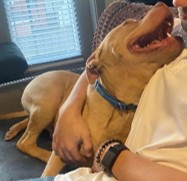
\includegraphics{final-report-images/nofacedog.jpg}
\caption{An Example of a Dog with their Face Obscured}
\label{fig:x dog no face}
\end{figure}
The second, is the by cropping the image to only the dogs face we theorize that valuable information is lost.  In the case of face verification in humans,only examining the face is reasonable and desirable because humans change clothes.  However, dogs do not.  We certainly note that there are cases where dogs do where clothes but these cases are infrequent.  Thus, we theorize that by leveraging a dogs entire dog we may see an improvement in the accuracy of the dog-identification model relative to work done by  Lai, Tu and Yanushkevich because the model could leverage additional characteristics such as the size of the dog.  This is illustrated in Figures \ref{fig:similar faces} and \ref{fig:different bodies} where in Figure 2 we see two dogs with similar faces.  One could forgive a model for classifying these dogs as the same.  But as shown in Figure 3 we can clearly see that are not.  By leveraging the entire body of dog, this miss-classification should be eliminated.

\begin{figure}[h]
\centering
	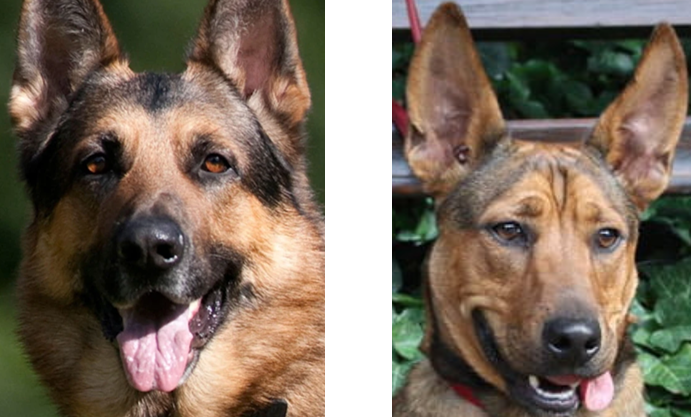
\includegraphics{final-report-images/similar_faces.png}
\caption{Sample Images of Two Dogs with Similar Faces}
\label{fig:x similar faces}
\end{figure}

\newpage

\begin{figure}[h]
\centering
	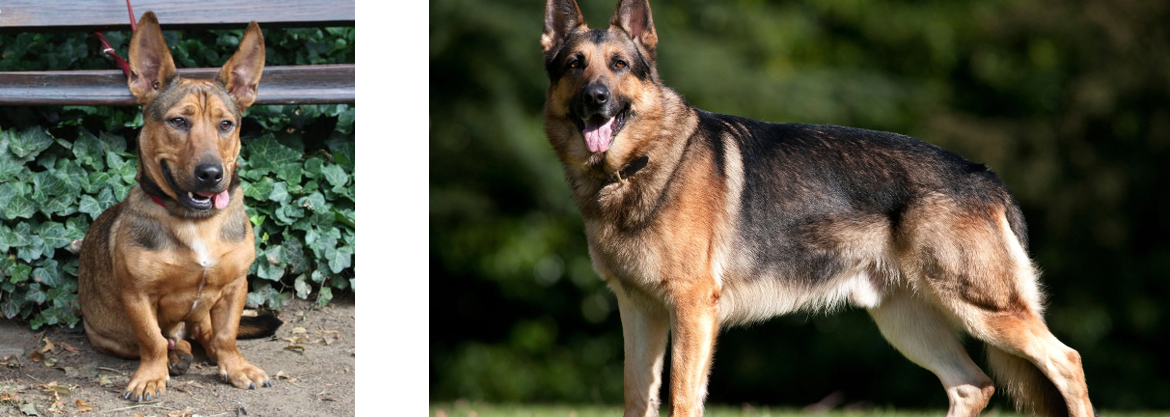
\includegraphics{final-report-images/different_bodies.png}
\caption{Sample Images of Two Dogs with Different Bodies}
\label{fig:x different bodies}
\end{figure}

Thus, we can now present the key problems this project aims to answer:

\begin{enumerate}
  \item By leveraging the entire body of a dog, can we construct an dog-identification model that can accurately determine if two dogs are the same or note?
  \item By removing the restriction of curated front facing dogs, can we construct a pipeline that can accurately match lost dogs with found dogs and vice versa? 
\end{enumerate}



\newpage
\section*{Bibliography}







\end{document}
